%Plagiarism checker http://smallseotools.com/plagiarism-checker/%
%Beautiful simple design for the web simulation%

%Easy table tool for latex http://truben.no/latex/table/

%Usefull diff tool online http://www.quickdiff.com/

%//

% Uncomment to activate the debug flag for debug mode:
\def\debug{}

\documentclass[12pt,MSc]{muthesis}
%{muthesis}
\usepackage[utf8]{inputenc}
\usepackage{graphicx}
\usepackage{url}
\urlstyle{sf}
\usepackage{caption}
\usepackage{subcaption}
\usepackage{color}
\usepackage{xcolor}
% META-TITLE INFORMATION
\title{Diabetic Avatar: Simulation of Behaviour in a 3D Virtual World \\-\\ Initial report}

\author{Assma Benharkat}
\date{May 10,  2013}

\makeatletter
% Comment to keep the chapter numbering: 
%\renewcommand{\thesection}{\@arabic\c@section}

\makeatother

\usepackage[a4paper, top=1.5cm, left=1.7cm, right=1.7cm, bottom=0.7cm, includehead, includefoot]{geometry}
%\usepackage{fullpage}

% Debug mode definition :
\newcommand{\warn}[1]{\ifdefined\debug\textcolor{blue}{#1}\else#1\fi}

\begin{document}

%%%%%%%%%%%%%%%%%%%%%%%%%%%%%%%%%%%%%%%%%%%%%%%%%%%%%%%%%%%%%%%%%%%%%%%%%%%%%%%%%%%%
%%%%%%%%%%%%%%%%%%%%%%%%%%%%%%%%%%%%%%%%%%%%%%%%%%%%%%%%%%%%%%%%%%%%%%%%%%%%%%%%%%%%
%\input{2-2II===Usecases}

%%%%%%%%%%%%%%%%%%%%%%%%%%%%%%%%%%%%%%%%%%%%%%%%%%%%%%%%%%%%%%%%%%%%%%%%%%%%%%%%%%%%
%%%%%%%%%%%%%%%%%%%%%%%%%%%%%%%%%%%%%%%%%%%%%%%%%%%%%%%%%%%%%%%%%%%%%%%%%%%%%%%%%%%%


\maketitle
   \begin{abstract}

%\warn{Corrected, but more content needed todo}\\
%One in ten people admitted to hospital in UK has diabetes.% 
Diabetes is the fifth most common cause of death in the world. The disease is accounted to be one of the most challenging health issues of the 21st century.  
%(Roglic G, Unwin N, Bennett PH et al (2005). The burden of mortality attributable to diabetes: realistic estimates for the year 2000. Diabetes Care 28;2130–2135)%
Experts estimate that diabetes treatment represents 10 \% of the National Health System budget. Besides, 
%=d'ailleurs, furthermore=en outre% 
treating diabetes complications cost 3 to 4 times more than normal diabetes treatment according to~\cite{LondonKanavos2012}. %A 2012 report from the London School of Economics, http://www.diabetes.co.uk/cost-of-diabetes.html%
\\A good diabetes management is essential to reduce these complications ~\cite{complications1993QuasiCours}, ~\cite{nathan2005intensive}
%NON CITE, nul car type 2 (Stratton IM, Adler AI, Neil HAW et al (2000). Association of glycaemia with macrovascular and microvascular complications of Type 2 diabetes (UKPDS 35): prospective observational study. BMJ 321; 405–412)%
and provides a better quality of life for patients. However, the management is not easy to achieve, as it requires daily injections, blood testing, and also an understanding of how glucose is used by their body.  
\\This reports describes an educational tool aimed at patients and their friends or family. Conceived as 3D simulation in a virtual environment, it will allow the user to play the role of a diabetic avatar that can walk, swim or perform any action that can be done in real world, while the impact of his lifestyle on his health can be studied. The simulation of the symptoms and the behavioural and heath impacts on the avatar are directly observed in-world, affecting the way a user explores the virtual world. 
\\The software presented in this document is a prototype based on Opensimulator, an open-source server platform for hosting virtual worlds, and represents my Msc final year project.


\end{abstract}

\tableofcontents

%%%%%%%%%%%%%%%%%%%%%%%%%%%%%%%%%%%%%%%%%%%%%%%%%%%%%%%%%%%%%%%%%%%%%%%%%%%%%%%%%%%%%%%%%%%%%%%%%%%%%%%%%%%%%%%%%%%%        CHAPTER 0   : Introduction                %%%%%%%%%%%%%%%%%%%%%%%%%%%%%%%%%%%%%%%%%%%%%%%%%%%%%%%%%%%%%%%%%%%%%%%%%%%%%%%%%%%%%%%%%%%%%%%%%%%%%%%%%%%%%%%%%%%%%%%%%%%%%%%%%%%%%%%%%%%%%%%%%%%%%%%%%%%%%%%%%%%%%%%%%%%%%%%%%%%%%%%%%%%%%%%%%%%%%%%%%%%%%%%%%%%%%%%%%%%%%%%%%%%%%%%%%%%%%%%%%%%%%%%%%%%%%%%%%%%%%%%%%%%%%%%%%%
\chapter{Introduction}
%Something like: "Diabetes is [lieu commun, blabla]. Puis diabetes et education" %sentence?
\section{Diabetes}
Diabetes is a disease characterized by a failure in the glycemic regulation system, when there is too much
sugar in the patient's blood. In a sound organism, energy can be used by the body when there is enough glucose and insulin. Glucose comes from eaten food, while insulin is a chemical hormone normally produced by the pancreas. In case of diabetes, there is no insulin (type 1) or the insulin cannot be used efficiently by the body (type 2). In this project, we will focus on type 1 diabetes, which was also called juvenile diabetes in the past as it's mostly diagnosed in children and young adults.\\There is still no cure for diabetes. However, patients can control their diabetes with different treatments. Treatment success relies mostly on the ability to manage one's own glucose levels. Therefore, patient education is crucial. 
When patients are diagnosed, they are educated about diabetes in the hospital during some days, and learn how to do blood testing and injections. Dietetic educational sessions are also hold, since some knowledge about food, energy and carbohydrate counting is needed directly after patients leave the hospital. Patient education continues for some months or even years in order to help them enhance their diabetes management.

\section{Simulations to enhance education}
A lack of education about diabetes can have fatal consequences, leading in some cases to coma
or death. We focus on teenagers education, accounted to be the most challenging to achieve because teenagers are known to be the hardest to teach. Indeed, as adolescence is a period where teenagers are progressively gaining their independence, they tend to consider adult's supervision as an annoyance.
%Hanna KM and Guthrie DW stated in [HG01]%

For this purpose, using a virtual environment to provide an immersive experience is expected to be much more effective, knowing the usual attractivity of gaming for a generation of teenagers more comfortable with a mouse than a pen in hand. 
%More used to mice than pens%

Simulations have been widely used for educational purposes. Two main uses of simulations can be distinguished: instructional simulations, that can be compared to lectures, and training simulations, similar to experimental sessions. We will see later that our tool enables both of these usages, depending on whether the user wants to acquire new knowledge or prefers experiencing the effects of diabetes on health in a safe environment.

As a comparison, teachers can experiment their teaching skills in a virtual classroom with simSchool rather than a real classroom, to avoid the risk of damaging real students. In this 3D realistic world, it would be possible to see how diabetes affects concretely the way patients live, work or do any other activity they usually do in real life. Patients can learn about their disease, and even experiment extreme %several%
behaviours to see both short term and long term consequences. For this purpose, time can be speeded up, to show things that cannot be experimented %by any practical or lecture% in real life.%, which they are supposed to avoid in real life for health reasons.%
\section{Opensimulator}
To develop such a 3D simulation, several alternatives can be considered. I studied them and a chose the most suitable in accordance with the constraints that will be discussed later.
Opensimulator is the virtual environment chosen to build this simulation. Among the famous virtual environments, we can cite Second Life developped by Linden Labs, and the game World of Warcraft. 
Opensimulator is similar to Second Life as people inside can owe virtual land, create objects, meet people and attend socializing events such as parties or concerts. The Opensimulator project was created in 2008 after the opensourcing of the 3D client of Second Life. Thus, a certain amount of interoperability between the two servers exists. Many universities created a virtual campus where lectures can be attended, and projects to train medical staff or run industrial simulations make a wide use of Opensimulator as it's an opensource software.
\\Opensimulator needs a client to connect to the server, as we need a browser to connect the web. A standalone version can also be used, in which case a local server %hosted in the user machine%
replaces the connexion to a distant server with the internet.

\section{Structure of this report}

First chapter is dedicated the literature review. Diabetes is explain more in detail, before reviewing existing attempts to model how diabetes works on glucose and insulin amounts and the most important contributions of software tools in the fields of diabetes monitoring and education. Second part of literature review stresses more on the close links between adolescence, diabetes and various issues as investigated in a large range of articles. This parts includes various subjects, from eating disorders to psychological and behavioural isssues, but most of them are linked with quality of life and education about diabetes. Such a large overview is needed in order to identify specific issues with diabetic teenagers, in order to figure out the more suitable approch that can be followed by the software. 
Second chapter presents the main advancements done in the project for various fields. We begin with a clarification of the requirements and needs that was made possible by the help of meetings with the diabetes team of Royal Manchester Children Hospital, and the newly diagnosed educational sessions I was allowed to follow in the hospital. After this, I describe the mathematical model of evolution of insulin and glucose concentrations in the blood. Then, a description of the technical choices made for the implementation is set, followed by the chosen architecture for the software. Last part presents the main developments that were done.
In the third chapter, the project plan is given, describing what is going to be implemented, software assessment and the principal milestones.
 
%\iffalse
\chapter{Litterature review}
% good graph for glucose and insulin effects after meals           http://en.wikipedia.org/wiki/File:Suckale08_fig3_glucose_insulin_day.png


% Aller voir les references du mail ayant pour objet "dissertation extract"


%wc latex: 
%begin  1606
%obj    
%end    

This chapter covers all the necessary background needed to understand the research, including a literature review and ``experimental’’ data about the material covered during diabetes educational sessions at the hospital.
\begin{itemize}
\item Section~\ref{sec:diab} explains what diabetes from a medical perspective (i.e. symptoms and treatments) and from a patient’s perspective, including psychological issues related to adolescence with diabetes and to diabetes management.
\item Section~\ref{sec:matmodel} describes various mathematical models that were developed to describe insulin and glucose evolution in the blood.
\item Section~\ref{sec:tools} provides an overview of existing tools for diabetes management and educational software.
\item Virtual environments and 3D simulations are covered in section~\ref{sec:VE}.
\end{itemize}


\section{Diabetes}
\label{sec:diab}
%%%%%%%%%%%%%%%%%%%%%%%%%%%%%%%%%%%%%%%%%%%%%%%%%%%%%%%%%%%%%%%%%%%%%%%%%%%%%%%%%%%%%%%%%%%%%%%%%%%%%%%%%%%%%%%%%%%%        CHAPTER 0   : A long term disorder                %%%%%%%%%%%%%%%%%%%%%%%%%%%%%%%%%%%%%%%%%%%%%%%%%%%%%%%%%%%%%%%%%%%%%%%%%%%%%%%%%%%%%%%%%%%%%%%%%%%%%%%%%%%%%%%%%%%%%%%%%%%%%%%%%%%%%%%%%%%%%%%%%%%%%%%%%%%%%%%%%%%%%%%%%%%%%%%%%%%%%%%%%%%%%%%%%%%%%%%%%%%%%%%%%%%%%%%%%%%%%%%%%%%%%%%%%%%%%%%%%%%%%%%%%%%%%%%%%%%%%%%%%%%%%%%%%%

% #ref Type 1 diabetes, novo nordisk%
Nothing can currently be done to prevent the onset of diabetes, and research still doesn't know exactly why the disease occurs. The immune system normally protects the body by destroying foreign substances such as bacteria. Diabetes develops when the immune system starts destroying the cells of the pancreas responsible for the creation of insulin. 

\subsection{A long term disorder}%"Biological side"%}
We assume that ``diabetes'' stands for ``type 1 diabetes'' in the following section. Diabetes occurs when the body stops producing insulin, usually without any early-warning sign in the case of type 1 diabetes. The young patient is often admitted to the hospital with a very high level of sugar in their blood, suffering from what is called hyperglycemia.

\subsubsection{Food and glucose regulation}
Glucose is an essential fuel for the \warn{body}, used by the organs such as muscles or the brain. Glucose comes from food and is released in the blood during digestion. Blood glucose control, is done by two hormones: insulin and glucagon. No matter the individual had a big meal a couple of hours before or fasted all the day, blood glucose is almost always between 4 and 7 mmol/L in non-diabetics. 
\\After a meal, blood glucose can rise up to 7.8 mmol/L. Insulin is then released, making the blood level decrease till it reaches a normal level, while the extra glucose is stored in the liver and the organs. When the level of glucose becomes too low, glucagon is produced, and some glucose contained in the liver is released in the blood.

%OK
\begin{figure}[h]
  \centering
  \caption{An example of insulin therapy: basal-bolus~\cite{bolusimage}}
  \includegraphics[scale=0.9]{Insulin_basal_bolus}\\
  ``The long acting insulin is given once (usually glargine, Lantus) or twice (usually detemir, Levemir) daily to provide a base, or basal insulin level. Rapid acting (RA) insulin is given before meals and snacks.''~\cite{bolusimage}
  \label{fig:Insulin_basal_bolus}
\end{figure}

\paragraph{Two insulins, two key functions}
%#ref nice graph p.20 of https://shop.diabetes.org.uk/usr/downloads/Carbs-Count-2012-reduced.pdf, can be used%
Insulin is an hypoglycemic hormone, which means that it makes blood glucose decrease. 
%Insulin is a hormone which is produced by the beta cells in the pancreas. Insulin acts like a key to unlock cells. It allows glucose in the blood stream to enter the cells. When insulin is not present, glucose cannot enter the cells and it builds up in the blood. %
We can see a common example of insulin therapy in figure~\ref{fig:Insulin_basal_bolus}, with the Basal Bolus Injection Regimen.
Basal insulin and bolus insulin are the two types used for diabetes treatment. Bolus insulin is injected after each meal in order to compensate the amount of glucose absorbed by eating. It's a short acting insulin. However, a minimal amount of insulin is needed all day long because organs need a little insulin to be able to convert glucose into energy. For this purpose, basal insulin is often injected once a day, it's a long acting insulin.

%However, insulin plays another key role: making the glucose usable by the organs. %
\subsubsection{Symptoms}
High blood glucose is called hyperglycemia, and is due to a lack of insulin. Thus, muscles cannot turn blood glucose into energy to use it, given that insulin is needed for this process. Hyperglycemia is characterized by %(an extreme) 
tiredness \warn{with a very high blood sugar}. The body reacts by trying to get rid of some glucose via the urines. Such a patient will need to drink large amounts of water and urinate unusually often. 

Low blood glucose is called hypoglycemia, and occurs mainly in diabetics because of too much insulin injected. The patient may feel dizzy, tired and can loose consciousness. Carbohydrates, often in the form of sugar, needs to be eaten quickly in order to raise blood glucose to a normal level.  

\subsubsection{Treatment and diabetes management}
Daily insulin therapy is the only way to treat diabetes. Patients need to learn how to inject, and how much insulin they inject. "Carbohydrate counting" is a technique used to match insulin requirements with food intake. The principles of carbohydrate counting will be explained in section~\ref{sec:ccount}.
%%%%%%%%%%%%%%%%%%%%%%%%    ADDED
%\section{Management WARNING: added and to be changed}
%"Management. The basic elements of type 1 diabetes management are insulin administration (either by injection or insulin pump), nutrition management, physical activity, blood glucose testing, the avoidance of severe hypoglycemia, and the avoidance of prolonged hyperglycemia or DKA." %in http://ndep.nih.gov/media/youth_factsheet.pdf
%%%%%%%%%%%%%%%%%%%%%%%

\subsubsection{Long term effects and complications}
High and low blood glucose can be corrected with insulin therapy. Living with poor blood glucose regulation has long term effects. Blood vessels are damaged, increasing the risk of heart diseases. Two other organs are often the first affected by long term high blood sugar, these are the eyes and feet. Sight loss and foot ulcers are more likely to occur if you have diabetes.  

\subsubsection{HbA1c}
HbA1c is used in diabetes management as an average blood glucose level. HbA1c stands for glycated haemoglobin, and is produced when glucose is fixed on haemoglobin molecules, which are the red blood cells in the blood stream. 
This value is different from blood glucose levels, which is a snapshot of the amount of glucose present in the blood at a given point in time. As red blood cells survive for 8 to 12 weeks, HbA1c is considered as an average measure of blood glucose. With the diabetes team, a patient tries to follow the target levels descibed in table~\ref{table:hba1cValues}.

\begin{table}
    \begin{tabular}{|l|l|l|}
    \hline
    Target Levels & HbA1c (\%) \\ \hline
    Non-diabetic          & 4 to 5.9\%                    \\ 
    People with diabetes and greater hypoglycemia risk           & 7.5\%    \\ 
    People with diabetes       & 6.5\%                     \\ 
    \hline
    \end{tabular}
    
    \caption{Target values for HbA1c}
    \label{table:hba1cValues}
\end{table}


HbA1c is stable over 3 months, so it's usually tested each 3 months if the patient wants to improve diabetes control, and every 6 months for routine examinations if diabetes control is good.



%%%%%%%%%%%%%%%%%%%%%%%%%%%%%%%%%%%%%%%%%%%%%%%%%%%%%%%%%%%%%%%%%%%%%%%%%%%%%%%%%%%%%%%%%%%%%%%%%%%%%%%%%%%%%%%%%%%        CHAPTER 0   : Psychological issues                %%%%%%%%%%%%%%%%%%%%%%%%%%%%%%%%%%%%%%%%%%%%%%%%%%%%%%%%%%%%%%%%%%%%%%%%%%%%%%%%%%%%%%%%%%%%%%%%%%%%%%%%%%%%%%%%%%%%%%%%%%%%%%%%%%%%%%%%%%%%%%%%%%%%%%%%%%%%%%%%%%%%%%%%%%%%%%%%%%%%%%%%%%%%%%%%%%%%%%%%%%%%%%%%%%%%%%%%%%%%%%%%%%%%%%%%%%%%%%%%%%%%%%%%%%%%%%%%%%%%%%%%%%%%%%%%%%
%\subsection{Enhancing diabetes management/"Psycological issues"}
\subsection{Psychological issues and diabetes management}

Adolescence represents a period of transition that brings about %OR (comes up with?) 
profound changes in a child's life, bringing physical, intellectual and psychological changes. Such changes are hard to deal with, and can be amplified by a conflicting relationship with parents. Being diagnosed with diabetes in such a period is especially challenging.
\\
For diabetics, adolescence with diabetes is complicated for several reasons. Physiological changes can induce insulin resistance, so patients with well managed diabetes can suddenly change to poorly controlled diabetes. Lack of well-being and psychological issues can seriously affect diabetes management. 
\\
\paragraph{Medical effects}
The hormones that causes growth during adolescence are also known to induce a insulin-resistance~\cite{HelpChildTeenTD1}.

%http://jdrf.org/life-with-t1d/type-1-diabetes-information/control-and-management/helping-your-child-or-teen-live-with-type-1-diabetes/

Growth Hormone, involved in the growth of bone and muscle mass during puberty, is thought to be responsible for this resistance. As a result, glucose levels tend to be higher, and insulin doses usually need to be increased to suit the patient's needs. 
%This results in highs and lows. 
Adrenaline worsens the situation as sudden falls in blood glucose trigger adrenaline emission, which results in the release of stored glucose. 
Experiencing such high variations in blood glucose often result in a strong feeling of loss of control.\\

Due to adolescence, nutritional requirements also change while the body experience the greatest amount of growth in height and weight. Daily food intake have to increase to meet the new body's needs, and teenagers often struggle with a hungry feeling between meals.  

%\paragraph{Management || treatment changes || treatment efficiency (adherence?)}
\paragraph{Adolescence and changes in diabetes management}
Due to this insulin resistance and the profound changes of adolescence, treatment need to be readapted, usually with higher insulin doses. Hypoglycemia can result, and a frustrating feeling of constant hunger. \\A good example of treatment adaption is the way practicians are recommanded to advise adolescents about snacking. \\
%REFERENCE Bon livre ! Pour des conseils, etc : http://books.google.fr/books?id=GVjW7m9cE1QC&pg=PA20&lpg=PA20&dq=adolescence+hunger+snack+diabetes&source=bl&ots=gGlnWXTytD&sig=VevM2h2Oy8Xe8a8uNMUO4P-0gR8&hl=fr&sa=X&ei=aJD3UbiGAseV7AbR94FY&ved=0CDoQ6AEwAQ#v=onepage&q=adolescence%20hunger%20snack%20diabetes&f=false
In order to reduce cravings between meals, practicians can advise teenagers about snacking. We can cite the use of free food, which is food with negligible amount of carbohydrates, ie 20 or less calories per serving. This kind of food can be reasonably consumed as often as wanted by the diabetic patient \cite{tu1993assessment}. However, the more adolescents are growing, the more energy they need, which makes free-food-based snacks inadequate. Thus, patients are advised to have a good-sized snack with an insulin injection in order to prevent lows and keep glucose levels under control, instead of simply taking only one small snack, and being hungry quickly after, or tacking multiple spaced snacks without insulin injections, resulting in hyperglyecmia risks. A good snacking policy is related with higher quality diabetes management, with lower HbA1c levels~\cite{delahanty1993role}, especially for snacks in the evening or consistent night snacks.
\\
On top of that, children and adolescents misconceptions about snacking need to be cleared to lead to good snacking habits. Usually, they all know that non-free-food snacks beyond the meal plan are not allowed by their caregivers. Considering it a ``bad'' behaviour, they tend not to mention extra-snacks when discussing their insulin plan with the diabetes team. Snacking is a good example of a kind of treatment change due to adolescence.

%=EFFICIENCY=
%* Motivational therapy : gives long term neutral (not positive) results on HbA1c at 36 months(Article "ismail2009motivational")Motivational enhancement therapy with and without cognitive behaviour therapy to treat type 1 diabetes: the long-term outcomes of a randomised controlled trial)
%=> A study performed on patients in 8 diabetes centres in the UK showed that a motivational behavioral therapy associated with a cognitive behavioural therapy resulted in an improvement of patient glycaemic control, with 50\% reduction of the HbA1c levels 12 months after the beginning of the study, compared to patients that were only provided with usual care. However, 24 months after the beginning of the study, there were no significant difference between the groups in HbA1c levels.
%The improvement due to the motivational and cognitive behavioural therapy disappeared after 24 months, so only short term effects of the therapy can be highlighted.


\paragraph{Psychological issues: depression and diabetes}
%=Gender=
%\\
%=Depression=
%\\
%*Effects of depression : depression and bad food habits (Article "ahola2009depression") Depression and sense of coherence are associated with food intake and compliance with dietary guidance in type 1 diabetes
%\\
Adolescence with diabetes is psychologically burdensome. 
\\
Research showed that the prevalence of depressed individuals is higher in a diabetic population (24\%) than in a non-diabetic population (17\%) in a 3,010 individuals study~\cite{goldney2004diabetes}. Moreover, suffering from diabetes and depression (all) together have important consequences on quality of life : if depression has a higher effect than diabetes on quality of life, the effect of diabetes with depression is higher than the combination of both. 
\\
While depression can be treated with good results by antidepressants~\cite{Goodnick2000}, negative effects were reported on glycemic control when they were used by diabetics ~\cite{Lustman2002917}. Complications due to the combination of diabetes and depression lead to very important costs : total health care for diabetics suffering from depression were 4.5 higher than those for diabetics without depression ~\cite{egede2002comorbid}.
\\
Furthermore, figures of depression associated with diabetes in youth are alarming~\cite{Grey2002907}:\\
``Children with diabetes have a two-fold greater prevalence of depression, and adolescents up to three-fold greater, than youth without diabetes.''\\
~\cite{ciechanowski2000}
Linked with a poorer metabolic control and serious long-term complications, depression may alter adherence~\cite{Lustman2002917} to the diabetic care and induce an insulin-resistance because of an hypersecretion of cortisol. % REFERENCE NEEDED Family and support seems to play a key role in depression associated with diabetes, so behavioral therapies, including family approaches, could prevent or treat efficiently depression for such patients.
\\
Finally, well being promotion and psychological follow-ups seem crucial in order to prevent this kind of complications when dealing with diabetic youngsters.\\


%=Self image=

%\paragraph{Social issues}

%Concerning psychological issues, associations between a better mental health, a better control of glucose values and a more positive approach to diabetes management are highlighted in~\cite{hackworth2013predictors}. A relashionship between risky behaviour and poor diabetes control was also found. 

%=Family support=
%\\
%=Peer relashionships=
%\\

%\subsubsection{Social and psychological issues}
\subsubsection{The lack of support and education about diabetes}
Family Support represents a key point of the success of diabetes management. A study~\cite{maas2013interrelationships} revealed that depression in teenagers is associated with poor blood glucose control and parenting stress. The relationship found in ~\cite{clayton2013impact}  goes beyond that, revealing that mother's depression affects more diabetes management than a teenager's own depressed feelings.
\\Thus, parents' education appears as a crucial point affecting diabetes management. However, 
this article~\cite{familyFactors} showed that the importance of peer support, especially for the mother is extremely important. Indeed, there was a close link between adolescents with good glucose control and the parent's feeling of being supported by their peers, especially among mothers. This can be explained by the fact that mothers that make the largest effort in diabetes management consider that the burden of diabetes is too high, and that they have this feeling of being not supported enough by peers. The study highlighted the fact that peers, which might be relatives or the parent's friends, are not educated enough about diabetes to be able to take care of the child. Therefore, all the responsability and efforts remains in the parent's hands. This situation is partly due to a lack of accessible solutions to educate such friends and relatives about diabetes. The software we aim to produce in this project may provide a solution for the general public.\\
            

%\subsubsection{Diabetes at School}




%%%%%%%%%%%%%%%%%%%%%%%%%%%%%%%%%%%%%%%%%%%%%%%%%%%%%%%%%%%%%%%%%%%%%%%%%%%%%%%%%%%%%%%%%%%%%%%%%%%%%%%%%%%%%%%%%%%%        CHAPTER 0   : Patient education                %%%%%%%%%%%%%%%%%%%%%%%%%%%%%%%%%%%%%%%%%%%%%%%%%%%%%%%%%%%%%%%%%%%%%%%%%%%%%%%%%%%%%%%%%%%%%%%%%%%%%%%%%%%%%%%%%%%%%%%%%%%%%%%%%%%%%%%%%%%%%%%%%%%%%%%%%%%%%%%%%%%%%%%%%%%%%%%%%%%%%%%%%%%%%%%%%%%%%%%%%%%%%%%%%%%%%%%%%%%%%%%%%%%%%%%%%%%%%%%%%%%%%%%%%%%%%%%%%%%%%%%%%%%%%%%%%%
\subsection{Patient education}

%This Msc project is led by the University of Manchester and the Royal Manchester Children’s Hospital. 

When a child is first diagnosed, it is admitted to the hospital for a few days, usually 3 to 6 days. Medical care is provided at the very beginning and during the stay according to the condition. At the same time, the diabetes team, including doctors, nurses and dieticians are meeting the patient regularly. 

\\
The nurse teaches the patient mainly about general knowledge concerning the disease, and all the practical knowledge to be able to practice self care diabetes management. A dietician focuses mainly on carbohydrate counting, and helps the child to figure out an appropriate diet, with advice on nutrition and sport.\\

\warn{Knowledge about diabetes is sometimes very weak, which won't allow patients to achieve a correct diabetes management. In ~\cite{herrejon2009creation}, wa can see how carbohydrate counting level can be extremely poor:\\ 
"A second skill activity provided a list of foods along with their portion size and asked participants to use the carbohydrate counting method to create an appropriate breakfast, lunch, and dinner, each containing four carbohydrate servings. Participants completed this task correctly 50\% for breakfast, 39\% for lunch, and 44\% for dinner on their first attempt. The percent correct increased to 60\% with repeated attempts for all three meals (data not shown)."\\}


%%%%%%%%%%%%%%%%%%%%%%%%%%%%%       WARNING IFFALSE
\iffalse


\section{Hba1c, complications, ketones ?}
The paper
~\cite{HBA1Ckilpatrick2012rise}
%%%%%%%%%%%%%%%%%%%%%%%%%%%%%%%

\subsubsection{In the literature}
\subsubsection{Education on the ward}
In order to get a better understanding of patient's experience and expectations, I went to the hospital to attend the educational sessions. I was taught as if I was a real patient, and invited to ask the questions a teenager could ask. Trying to react as a ``normal'' patient was a way to collect the amount of knowledge they have, and the approach that is used to teach them.
\\In Royal Manchester Children’s Hospital, there is 4 sessions, 2 with the diabetes nurse, and 2 with the dietician. It may be underestimating to say that patients are often upset while they attend these sessions because they learnt only one or two days before that they were suffering from diabetes, a long term disorder.

%%%%%%%%%%%%%%%%%%%%%%%%%%%%%%%%%%%%%%%%%%%%%%%%%%%%%%%%%%%%%%%%%%%%




%%%%%%%%%%%%%%%%%%%%%%%%%%%%%       WARNING IFFALSE
\fi

%%%%%%%%%%%%%%%%%%%%%%%%%%%%%%%%%%
%%%     Carbohydrate counting
%%%%%%%%%%%%%%%%%%%%%%%%%%%%%%%%%%
\subsection{Carbohydrate counting} 
\label{sec:ccount}
This technique is used to manage blood glucose. \paragraph{Carbohydrate} is a nutrient, contained in some food and drink. During digestion, carbohydrate breaks down into glucose, which is then used as energy by the body. 
We can classify carbohydrates in two main types: starchy carbohydrates and sugars. 
"Starchy carbohydrates" come from sources such as pasta, bread, rice and potatoes. "Sugars" designate sucrose, fructose (found in fruits) and lactose (found in dairy foods). Patients need to take bolus insulin to cover the glucose derived from carbohydrates during meals~\cite{carbcountPdf}. 
\paragraph{}To find how much bolus insulin they need to take, diabetics should know:
\begin{enumerate}
\item How much insulin is needed for a certain amount of carbohydrates. This ratio is individual to each person, and tends to increase during adolescence.
\item The amount of carbohydrates they will eat and drink for this meal.
\end{enumerate}

%OK
\begin{figure}[h]
  \centering
  \caption{Example of a meal with corresponding carbohydrate levels~\cite{refhowtocarbPic}}
  \includegraphics[scale=1.2]{mealcount}
  \label{fig:mealcount}
\end{figure}

%Nice example in page 30 of the book%
For instance, if a patient has:
\begin{itemize}
\item A ratio of 1:10, which means that 1 unit of insulin is needed to cover 10 grams of carbohydrates in food
\item The food as shown in figure~\ref{fig:mealcount} as a meal
\end{itemize}



He will then sum the carbohydrates of the meal as follows:

$\begin{array}{l l l}
    Carbs & \quad  = 0 + 15 + 15 + 4 + 12   & \quad \textrm{Carbs in eggs, raspberry, bread, peanut butter and milk}\\
         & \quad = 46 g   
  \end{array}$
  
\paragraph{}
The ratio of 1:10 gives the units of insulin needed with a simple division of the total amount of carbohydrates by the ratio, rounded to the nearest whole number, as follows:

$\begin{array}{l l l}
    InsulinUnits & \quad  = 46/10 \\
         & \quad = 4.6  \\
         & \quad 5 units & \quad \textrm{rounded value}
  \end{array}$
\paragraph{}
In this example, 5 units of bolus insulin need to be injected. 

\paragraph{Correction doses of insulin} are added to the injection if blood glucose is high compared to the target values in table \ref{table:targetValues}. This may occur if the patient didn't take enough insulin before the previous meal or had some snack between two meals. Most people will need 1 unit of bolus insulin to reduce blood glucose levels by 2–3 mmol/l ~\cite{carbcountPdf}. 


\begin{table}
    \begin{tabular}{|l|l|l|}
    \hline
    Target Levels by Type & Before meals (pre prandial) & 2 hours after meals (post prandial) \\ \hline
    Non-diabetic          & 4.0 to 5.9 mmol/L           & under 7.8 mmol/L                    \\ 
    Type 1 diabetes       & 4 to 7 mmol/L               & under 9 mmol/L                      \\ \hline
    \end{tabular}
    
    \caption{International Diabetes Federation's target ranges for people with and without diabetes}
    \label{table:targetValues}
\end{table}


\paragraph{}In the previous example, if blood glucose before the meal was 10 mmol/L, and the patient's target value is 6 mmol/L. If one unit of insulin lowers the blood glucose levels by 2 mmol/L, the target is to lower the blood glucose by 4 mmol/L. Thus, 2 units of insulin will reach the target level.
\\This corrective dose of insulin needs to be added to the insulin counted by the carbohydrate couting method, so the toal amount of injected insulin is 5 + 2 = 7 units of insulin.

\paragraph{How to know the amount of carb in a meal ?}
There are various ways to figure out the amount of carbohydrates available in a given food:
\begin{itemize}
\item The patient can read food labels, where the amount of carbohydrates for 100g or for a given portion is indicated.
\item Reference lists can be used. These lists are available in some leaflets provided by the hospital, and in the very comprehensive reference book~\cite{cheyette2010carbs} given to each newly diagnosed patient. 
%screen book https://shop.diabetes.org.uk/usr/catalogue/pi_442.jpg
\end{itemize}

In the children's hospital, this book is widely used because portion sizes in a standard size plate are shown in pictures, which makes it really easy to find the correct amount by visual comparizon as can be seen in figure~\ref{fig:bookImage}. A mobile application~\cite{carbcalsAppWebsite} using this principle is also available for iPhone, Android and BlackBerry. Using easy-to-learn and visual methods fits the needs of diabetes management for young patients.
%OK
\begin{figure}[h]
  \centering
  \caption{Carb and Cals~\cite{cheyette2010carbs} book, used to figure out carbohydrates by visual comparizon}
  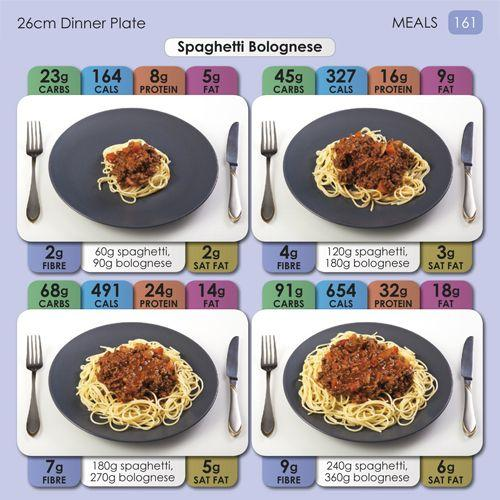
\includegraphics[scale=1.2]{bookImage.jpg}
  \label{fig:bookImage}
\end{figure}

%%%%%%%%%%%%%%%%%%%%%%
\warn{\subsubsection{Glycemic Index and Glycemic Load}}
 %TAKEN from implementation, feeding system\\

\label{sec:GIGL}

\iffalse
%Recopier le tableau en latex si j ai du temps
\begin{figure}[h]
  \caption{Carbohydrates in a set of food servings - Adapted from \cite{foodGlucoseTableWebsite}}
  \centering
  \includegraphics[scale=0.6]{foodGlucoseTable}
  \label{fig:foodGlucoseTable}
\end{figure}
\fi

\\
\warn{Using the Glycemic Index (GI) and the Glycemic Load (GL) can help diabetics to predict blood glucose variations. Used by nutritionists since 1980, the glycemic index characterizes how quickly blood glucose rises after the consumption of a specific kind of food. 
The GI is based on a reference, usually pure glucose or white bread, valued at 100 which is the highest possible GI as shown in figure~\ref{fig:low-high-GI}. 30 minutes after the food consumption, a higher GI induces a higher blood glucose peak. It can also be noticed that if the GI is between medium and high, an reactive (or postprandial) hypoglycemia is observed after 2 hours, which wouldn't be observed if the consumed food had a lower GI.}

\iffalse
%cited ?
\begin{figure}[h]
  \caption{Glycemic index for different kind of food}}
  \centering
  \includegraphics[scale=0.6]{}
  \label{fig:}
\end{figure}
\fi

%tocite
\begin{figure}[h]
  \caption{Low and high GI \cite{last2006low}}}
  \centering
  \includegraphics[scale=0.6]{GI_two_curves}
  \label{fig:low-high-GI}
\end{figure}

\warn{If the temporal rise of blood glucose can be predicted by using GI, this index doesn't take into account the amount of ingested carbohydrates. For this purpose, the glycemic load (GL) was established to estimate how much the blood glucose will rise after eating a specific food. Knowing the food serving weight and the amount of glucose inside, this formula gives the link between the glycemic index and the glycemic load: $GL = IG * (mglucose/mfood)$ where mglucose and mfood are the glucose mass and the insulin mass, in grams.}
\\
\warn{Figure~\ref{fig:GL_and_GI-Chart} shows the possible values for the GI and the GL.}


\iffalse
\begin{figure}[h]
  \caption{Glycemic index and glycemic load values, from \cite{mendozaWebsite}}}
  \centering
  \includegraphics[scale=0.6]{GL_and_GI-Chart.gif}
  \label{fig:GL_and_GI-Chart}
\end{figure}
\fi
%%%%%%%%%%%%%%%%%%%%%%


\subsection{Motivations}
Remove ?
\warn{Intensive diabetes treatment has positive consequences on the onset and evolution of complications, postponing them~\cite{dcct1994effect}. Rethinopathy occurence was reduced by 53\% for patients followed on average for 7.3 years. On the other hand, patients that followed normal therapy without specific glycemic targets and patients following an intensive therapy that aimed for a near-normal glycemic level with 3 or more insulin injections a day were fewer than 1\% to have an amputation or become blind because of diabetes. [explain somewhere more in detail, with the figures, and keep only the summary here]

"Moreover, suboptimal glycemic control that is established during early adolescence[3] may be very difficult to change, even with state-of-the-art behavioral intervention.[4]"}

\section{Virtual Worlds}

\subsection{Definition}
Defining virtual worlds is not easy. Since the early 80's, many definitions were given, closely linked with the technical evolutions in computer science~\cite{warburton2009second}. %Can be cited [warburton2009second] : check what i'm citing here ! 

\begin{figure}[h]
  \caption{A virtual auditorium in Second Life ~\cite{ref_VE_audit}}
  \centering
  \includegraphics[scale=0.6]{VE_auditorium.jpg}
  \label{fig:VE_audit}
\end{figure}

%Common recurrent patterns were identified, linked with synchronicity, persistance, avatar representation and network of users. 

One of the simplest approaches is to describe Virtual Environments in terms of a technological environment that make the user strongly feel that he is "present in an environment other than the one [he is] actually in", and compelled to "interact with that environment"~\cite{schroeder1996possible}. This kind of environment can find many usages, such as providing an environmement in order to realize tasks that cannot sometimes be made possible in real life, whether it's because the task cannot be done, given the existing physical constraints (flying, for instance). An historical, but still current use of virtual environments is to set classrooms or meetings, gathering virtually people that are in different places in real life. The virtual platfrom can provide a way to communicate, either by text, voice or video as shown in picture~\ref{fig:VE_audit}. The feeling of being present in the virtual environment is reinforced by being able to see exactly how many participants are sitting there, and even to interact with them, like shaking hands, or the ability to give other people virtual objects.

%[found in: Second Life in higher education: Assessing the potential for and the barriers to deploying virtual worlds in learning and teaching].


\subsection{A classification of virtual environments}
Multiplayer online games such as World of Warcraft were a major influence of modern virtual environments. Thus, commons features are shared, like the avatars that can be personalized as humanoid representations of the users in ~\ref{fig:VE_wow}.
Persistancy of the environment, interactions between multiple users, objects that can be owned and used, and an explorable world that presents similarities to the real world (physics, maps), enforcing the illusion of being in the game are other features commonly shared by this kind of games and virtual environments~\cite{warburton2009second}. 

\begin{figure}[h]
  \caption{World of Warcraft : Creation and personalization of an avatar~\cite{ref_VE_wow}}
  \centering
  \includegraphics[scale=0.7]{wow.jpg}
  \label{fig:VE_wow}
\end{figure}



\paragraph{}
Multiple classifications of Virtual environments were developped. A topology based on~\cite{mckeown2007taking} divided virtual environments in 4 main categories~\cite{warburton2009second}:
\begin{itemize}
\item Flexible narrative : Massively Multiplayer Online (MMO) games and serious games. Includes a scnearized evolution and goals to achieve.
\item Virtual social world : Social platforms, 3D chat rooms. Communication and socialization are especially emphasized, and there is no specific aim.
\item Simulation : simulations of the real world, such as Google Earth. Specific simulation needs are adressed, often for scientific or technical purposes. No inworld avatars, unless rare exceptions.
\item Workspace : 3D computer-supported workspaces. Commonly multiuser, with specific tools included according to the public aimed.

\end{itemize}

We will focus on multi-user virtual environments (MUVEs), which include the Social World and the Workspace categories. 
%MUVEs share many common features with massively multiplayers online games (MMOs) such as World of Warcraft. 


\subsection{Second Life}

Many virtual social worlds have an important community, among which Habbo, one of the oldest ones with 90 million users (Kzero Worldswide, 2009) and the famous Second Life, released in 2003~\cite{wang2009extending}. 
%Or cite this (guillet2013conducting): As of January 2010, over 162 million avatars have been registered to Habbo Hotel and there are an average 16.5 million unique visitors monthly (Sulake, n.d.).
\paragraph{}
It's is the most famous example of virtual environments, where avatars can explore the world by walking, flying and can create, use and sell objects. The example of second life make it clearer that virtual environments are not games, as there is no specific aim or storyline in-world. Socialization is a key issue, and every kind of real life activity can be done in-world, like swimming, dancing in parties or shopping in big malls created and owned by users.
  
%The kind of environment were are interested in Second Life, released in 2003~\cite{wang2009extending} is the most famous example of virtual environments, which . %

\input{1-2Modelbergman}
\input{1-3Tools}
%\fi

%wc V matin: 272 IRL

%\chapter{Analysis}
\input{2-1diabetes-sessions}
\input{2-2I===Aims}

%\chapter{Design}
\input{2-2II===Usecases}
%\input{2-3Architecture}
%add links between sections
%\subsection{Django web server}
Used for 3 taks : 
\begin{enumerate}
\item The Energy Bar displayed in world. 
% PUT IN MY WORK : It looks like a progress bar indicating the amount of left energy for the avatar (or glucose in the avatar's blood). The energy indicator consists on an dynamic webpage rendered by the web server and displayed on an object in world. 
\item The glucose graph.
\item A history of each time the avatar used a glucose-meter to test blood, and the corresponding  values.
\end{enumerate}

\subsubsection{Energy Bar}
Using an SQLite database to store the data.
Writting a model. For the energy indicator, an object with the energy value associated with the corresponding time and date are needed. In the file '1energy.py', an EnergyLog class is created, with an integer and a date field.
Writting the view. The view is any function called by the server, and is used to render a webpage as a result of a request. In the file 'views', a method 
%\input{2-4Modelimpl}
%\input{2-5scripts}


%\iffalse
\chapter{Project Plan}
\input{3-1Steps}
\section{Gant Diagram}
\includegraphics[scale=0.5]{gantt3.png}\\
Main tasks are in dark green, subtasks in pale green and optional tasks in briliant green (with \# marks).
Tasks in red are likely to change depending on how meetings can be scheduled with diabetic patients.
\section{Reflexions about previous project plan}
Considering the previous Gantt diagram, we can see that milestones that were determined in the initial report were respected and are still available. This can be accounted to the fact that exams and meetings with the staff were taken into account. For the elaboration of this version, some facts were taken into account in order to avoid irrealistic milestones. For instance, some facultative fonctionalities can be developped before finalizing each version. This will allow us to meet our deadlines even if the development is slower than expected.
\\Time for the elaboration of the questionnaire was also allowed in the middle of the period where version 3 will be developped, because the questionnaire should be ready before the end of 3rd version development, but can be done too early while some feedback from the hospital (after demonstrating version 2) is needed to design the questionnaire.
%\fi


\chapter{Real implementation}
\input{4-1Opensim}
\subsubsection{More realist/handy : Adding "wash hands / take a bath" instead of Sit text}
Only if used, or if nothing better
\subsubsection{More intuitive UI : Changing the onClick logo}
URL : % http://wiki.secondlife.com/wiki/LlSetClickAction/fr

%%%%%%%%%%%

\subsection{Food system}

\subsubsection{General overview}
The implementation of a food system that allow the representation of a diabetic avatar was designed following the created model described in section~\ref{sec:mymodelSection} and was made as generic as possible so that the model can be easily enhanced or changed.

At each time, glucose level can be computed from the model according to global and local parameters as shown in figure~\ref{fig:GLparam}. These parameters are located in two scripts : StateScript and FoodObject. As described in section~\ref{}, StateScript is the main script for the avatar, controlling the glucose-insulin system and the avatar's behaviour related to diabetes such as triggering hypoglycemia or hyperglycemia symptoms. FoodObject is a generic script that describes each food item behaviour. 

According to our requirements, a minimal amount of specific features need to be implemented for each kind of food : the total amount of glucose in a food item, the time needed to reach the glucose peak (maximum level of blood glucose since the food consumption). This generic skeleton is used for each food object in the simulation. The total amount of glucose is taken from tables such as~\ref{fig:foodGlucoseTable} and \cite{nutritiondataWebsite} %http://nutritiondata.self.com/ 
when the data can't be found in other tables. 
\\
The Glycemic Index (GI) and the Glycemic Load are two measures %values
that can be found in such tables. Used by nutritionists since 1980, the glycemic index characterizes how quickly blood glucose rises after the consumption of a specific kind of food. 
Created in the 1980s, the GI is based on a reference, usually pure glucose or white bread, valued at 100 which is the highest possible GI as shown in figure~\ref{manyIG}. 30 minutes after the food consumption, a higher GI induces a higher blood glucose peak. It can also be noticed that if the GI is between medium and high, an reactive (or postprandial) hypoglycemia is observed after 2 hours, which wouldn't be observed if the consumed food had a lower GI.

If the temporal rise of blood glucose can be predicted by using GI, this index doesn't take into account the amount of ingested carbohydrates. For this purpose, the glycemic load (GL) was established to estimate how much the blood glucose will rise after eating a specific food. Knowing the food serving weight and the amount of glucose inside, this formula gives the link between the glycemic index and the glycemic load : $GL = IG * (mglucose/mfood)$
\\

\paragraph{Food object : providing a realistic experience}
\label{sec:food}
The food object is an object that represents a food item in 3D, with a script inside to make the object eatable. The food object doesn't do any calculation, but sends to the StateScript the reference values that correspond to the food. The main issue to solve with the script object was to give it a realistic behaviour. 
\\

To trigger the action of eating the food, different solutions are possible : 
\begin{enumerate}
\item The food is eaten when the avatar right-clicks on the object to access the contextual menu, then selects the "Eat" action. The addition of personalized commands in the contextual menu was needed in some other cases, and the solution to make it is explained in section~\ref{sec:menuAction}. 
\item The food is eaten when the avatar "walks" on the object, as in some video games.
\item The food item is eaten when the avatar simply clicks on it. A minor problem with this solution is that there is no way to know in advance which object is "eatable" if there's nothing to show it's clickable, like a different mouse icon. As I planned to remove the text written on the food, it will be hard to detect with which object of the kitchen interactions are available.
\end{enumerate}
Maybe explain pros and cons of each, and why I finally choose this one. %TODO : finish

\paragraph{Different animations : an animation library (generalize it for the insulin injection ?)}
\label{sec:animLib}

According to the food objects nature, the eating animation played will be different. In fact, eating a sandwich is different of eating a bit of chocolate: in the first case, the two hands may be needed, and the animation takes longer as eating a sandwich takes more time, while in the second case, only one bite is needed.

2 kinds of elementary animations were used : 
-for single item/simple bite and for plate
-for drinking

The idea was to loop them for food objects that need many bites. By combination, the simple bite animation could be used for many purposes :
-to eat a simple item, like a crisp
-combining a right hand simple bite animation with a left hand one to eat sandwiches
-adding another animation for cutting food in a plate/taking a piece of food in a plate, and then playing the simple bite animation.

For drinking, the animation was simply looped.

\paragraph{Food detruction}
\label{foodDestruction}
Food destruction needed to be considered at the very beginning, because after being called by the script, the llDie() function interrupts the execution of the script. As a consequence, the food script cannot ensure the progressive release of glucose in the avatar's blood over the time, that is supposed to last about 2 hours. 
Moreover, the destruction of the food object need to be synchronized with the end of the eating animation : if the objects dies too early, the avatar will appear as eating nothing, and if it dies too late, the food item will disappear unrealistically after the end of the eating movements, while being in the hand. If possible, the food object should die when it's close to the mouth, during the latest bite. As all food items are not using the same animation while being eaten as described in section ~\ref{secDiffAnim} , the duration of the animation also needs to be stored, as an internal value for the Food script, for each kind of food. With this information, the llSleep function can be called by the script to stop its execution during the animation, waiting for the appropriated moment to kill the object. 
Computing the appropriate moment was complicated by the rights permission that asks the user allows the food attachment to his hand, triggered after clicking on the food item. This time need to be added to the computation. Moreover, the issues explained in section~\ref{sec:animLib} about playing multiple animations or looping them need to be taken into account, and need to be added to the result. Graph of the execution ? With one or two animation shown. %The animation lenght is automatically computed ... do it ?


\paragraph{Adding an action in the contextual menu}
\label{sec:menuAction}
We can add a personalized action to be executed when selected in the contextual menu~\ref{contextMenu}. The added action will replace the original default action, a "Sit" action that makes the avatar sit on the object. It is a default action allowed for any physical object by Opensim, even if the sitting action and the sitting point (see section~\ref{sittingpoint} for details on the sitting point) aren't already defined by the user for the object. 
\\For some reasons, we may want to make another action available from the contextual menu instead of the Sit action. The number of buttons in the contextual menu is fixed, so the only way to do so it to replace the Sit button. First step is to change the action executed when clicking on the button. This can be done by scripting, calling the 
llSetSitText

\subsubsection{Orientation and position issues related to the animation's constraints}

\paragraph{A position issue: the exemple of the fishing activity}
\label{sittingpoint}

Set the fishing animation.
The sitting point has to be defined, which means that any time someone sits on the boat, the avatar will be sitting at the same point, with the same body orientation. If not defined, the sitting point can be anywhere on the boat as shown in figure~\ref{fig:goodSittingPoint, fig:wrongSittingPoint}, which means that the avatar position won't match the animation. It is an important issue because there won't be any realism in this case, and the user may even not recognize the played animation.

\paragraph{An orientation issue: the Eating example}
When eating a food item as described in section~\ref{sec:food}, the food item is put in the avatar's hand, and the corresponding animation is played. For this purpose, the food item need to be placed correctly in the hand, to make it realistic. However, as shown with the glass in figure~\ref{fig:badFoodOrientation, fig:goodFoodOrientation}, this position is often not compatible with the one originally used to display the food in world, here a glass placed upright on the table.
For this purpose, two solutions can be used : 
\begin{enumerate}
\item Changing the object's position by using the llSetPosition~\cite{llSetPositionWebsite} in a script to change the orientation of the object depending on whether it is attached to an avatar or on the table. 
\item Using a "display only" object that is also used for automatic objects creation. The idea here is, for a set of brownies for instance, to create an "aggregate" of brownies, such as 7 or 8 pieces of cake on a plate.
This solution is especially convenient for some kind of food items, as it provides a way to generate automatically food when it is used. Disadvantage : the solution doesn't work for any kind of objects : creating an aggregate of pasta plates is not a good solution because a user usually wants to eat one item of this kind of food. There is also a problem as the food won't disappear from the plate when taken and eaten, which might look weird for an aggregate with a small number of objects displayed.  
The aggregate is created by arranging several food objects in the desired display, and then linking them into a "super object", the aggregate. As shown in figure~\ref{fig:aggregate}, Opensim make the aggregate appear as a single object. Thus, normal properties of objects are usable, in particular the object's inventory. Other objects can be put in the inventory and used by the scripts, so the object we want to give to the avatar (for instance, a piece of brownie with the orientation that matches the eating animation with the brownie held in the avatar's hand) can be put in this inventory and given by the main script of the aggregate to the avatar. The attachToAvatar~\cite{llAttachToAvatarWebsite} function is called for this purpose, and gives a copy of the brownie in the aggregate's inventory to the avatar. 
\end{enumerate}

Maybe explain when each solution is better and when I also used them ?


\subsection{Energy intake}
-speed+simultaneousFood
-insulin


Computation : 
 
-Energy intake
    *generic skeleton
    *speed
    
-Realistic system :
    A) food need to disappear : 
        1)was a problem : how to add energy continuously if the object that contained the food script died ? 
        2)wait a fixed amount of time (depending on the kind of objects, how long it's supposed to take to eat it) before being destroyed.
        
    B) food animation : the avatar have to seem realistically eating the food item. Thus :
        1) different kind of animations for different kind of food. 3 main animations : eat a normal item, like a cake, drink, or eat like a sandwich.
        2) food orientation issue : it was an important issue... Use a distributor object cf "Giving objects" subsection
    
    C) supporting simultaneous food items eaten when an "active period" can overlapp.
    D) Food name written from the script


%%%%%%%%%%%%%%%%%%%%%%%%%%%%%%%%%%%%%%%%%%%%%%%%%%%%%%%%%%%%%%%%%%%%%%%%%%%%%%%%%%%%%%%%%%%%%%%%%%%%%%%%%%%%%%%%%%%         CHAPTER 1   : State of the art    %%%%%%%%%%%%%%%%%%%%%%%%%%%%%%%%%%%%%%%%%%%%%%%%%%%%%%%%%%%%%%%%%%%%%%%%%%%%%%%%%%%%%%%%%%%%%%%%%%%%%%%%%%%%%%%%%%%%%%%%%%%%%%%%%%%%%%%%%%%%%%%%%%%%%%%%%%%%%%%%%%%%%%%%%%%%%%%%%%%%%%%%%%%%%%%%%%%%%%%%%%%%%%%%%%%%%%%%%%%%%%%%%%%%%%%%%%%%%%%%%%%%%%%%%%%%%%%%%%%%%%%%%%%%%%%%%%
%OLD \chapter{State of the art} % or Background research}%

%%%%%%%%%%%%%%%%%%%%%%%%%%%%%%%%%%%%%%%%%%%%%%%%%%%%%%%%%%%%%%%%%%%%%%%%%%%%%%%%%%%%%%%%%%%%%%%%%%%%%%%%%%%%%%%%%%%         CHAPTER 2   : Diabetes    %%%%%%%%%%%%%%%%%%%%%%%%%%%%%%%%%%%%%%%%%%%%%%%%%%%%%%%%%%%%%%%%%%%%%%%%%%%%%%%%%%%%%%%%%%%%%%%%%%%%%%%%%%%%%%%%%%%%%%%%%%%%%%%%%%%%%%%%%%%%%%%%%%%%%%%%%%%%%%%%%%%%%%%%%%%%%%%%%%%%%%%%%%%%%%%%%%%%%%%%%%%%%%%%%%%%%%%%%%%%%%%%%%%%%%%%%%%%%%%%%%%%%%%%%%%%%%%%%%%%%%%%%%%%%%%%%%
%OLD \input{3Diabetes}
%%%%%%%%%%%%%%%%%%%%%%%%%%%%%%%%%%%%%%%%%%%%%%%%%%%%%%%%%%%%%%%%%%%%%%%%%%%%%%%%%%%%%%%%%%%%%%%%%%%%%%%%%%%%%%%%%%%%        CHAPTER 3   : (An instructional and training) Simulation Tool    %%%%%%%%%%%%%%%%%%%%%%%%%%%%%%%%%%%%%%%%%%%%%%%%%%%%%%%%%%%%%%%%%%%%%%%%%%%%%%%%%%%%%%%%%%%%%%%%%%%%%%%%%%%%%%%%%%%%%%%%%%%%%%%%%%%%%%%%%%%%%%%%%%%%%%%%%%%%%%%%%%%%%%%%%%%%%%%%%%%%%%%%%%%%%%%%%%%%%%%%%%%%%%%%%%%%%%%%%%%%%%%%%%%%%%%%%%%%%%%%%%%%%%%%%%%%%%%%%%%%%%%%%%%%%%%%%%


%%%%%%%%%%%%%%%%%%%%%%%%%%%%%%%%%%%%%%%%%%%%%%%%%%%%%%%%%%%%%%%%%%%%%%%%%%%%%%%%%%%%%%%%%%%%%%%%%%%%%%%%%%%%%%%%%%%%        CHAPTER 4       %%%%%%%%%%%%%%%%%%%%%%%%%%%%%%%%%%%%%%%%%%%%%%%%%%%%%%%%%%%%%%%%%%%%%%%%%%%%%%%%%%%%%%%%%%%%%%%%%%%%%%%%%%%%%%%%%%%%%%%%%%%%%%%%%%%%%%%%%%%%%%%%%%%%%%%%%%%%%%%%%%%%%%%%%%%%%%%%%%%%%%%%%%%%%%%%%%%%%%%%%%%%%%%%%%%%%%%%%%%%%%%%%%%%%%%%%%%%%%%%%%%%%%%%%%%%%%%%%%%%%%%%%%%%%%%%%%
%OLD\input{5WorkDone}

%%%%%%%%%%%%%%%%%%%%%%%%%%%%%%%%%%%%%%%%%%%%%%%%%%%%%%%%%%%%%%%%%%%%%%%%%%%%%%%%%%%%%%%%%%%%%%%%%%%%%%%%%%%%%%%%%%%%        CHAPTER 5       %%%%%%%%%%%%%%%%%%%%%%%%%%%%%%%%%%%%%%%%%%%%%%%%%%%%%%%%%%%%%%%%%%%%%%%%%%%%%%%%%%%%%%%%%%%%%%%%%%%%%%%%%%%%%%%%%%%%%%%%%%%%%%%%%%%%%%%%%%%%%%%%%%%%%%%%%%%%%%%%%%%%%%%%%%%%%%%%%%%%%%%%%%%%%%%%%%%%%%%%%%%%%%%%%%%%%%%%%%%%%%%%%%%%%%%%%%%%%%%%%%%%%%%%%%%%%%%%%%%%%%%%%%%%%%%%%%


%%%%%%%%%%%%%%%%%%%%%%%%%%%%%%%%%%%%%%%%%%%%%%%%%%%%%%%%%%%%%%%%%%%%%%%%%%%%%%%%%%%%%%%%%%%%%%%%%%%%%%%%%%%%%%%%%%%%        CHAPTER 6       %%%%%%%%%%%%%%%%%%%%%%%%%%%%%%%%%%%%%%%%%%%%%%%%%%%%%%%%%%%%%%%%%%%%%%%%%%%%%%%%%%%%%%%%%%%%%%%%%%%%%%%%%%%%%%%%%%%%%%%%%%%%%%%%%%%%%%%%%%%%%%%%%%%%%%%%%%%%%%%%%%%%%%%%%%%%%%%%%%%%%%%%%%%%%%%%%%%%%%%%%%%%%%%%%%%%%%%%%%%%%%%%%%%%%%%%%%%%%%%%%%%%%%%%%%%%%%%%%%%%%%%%%%%%%%%%%%
%\chapter{Summary}
%Simulations have been widely used in the contect of education. 
%
%We saw in the literature review that an effective diabetes management can reduce diabetes complications. Technology  cannot be isolated from educational issues, psychological condition o how contribution
%
%Design of 
%
%Limits of the project have been set 
%
%
%Advancement in today’s technology means that there are fewer barriers to education. Second 
%Life (SL), currently being the most well-known virtual world platform could do well in 
%aiding this purpose. However, SL is a commercial version that requires some amount of cost. 
%OpenSim, which is the open source version, would be better to suite this purpose because it 
%requires less cost and since it is open source, it encourages developers to extend the version 
%and make it better to suite education purposes. Sloodle, a combination of OpenSim and 
%Moodle is one example of extended version of OpenSim that is helpful in learning especially
%in distance learning. Sloodle not only allows educators to teach using the virtual world but to 
%also monitor and assess students using the Moodle extension. However, technology alone 
%would not give much benefit if the content of the teaching material in the virtual world is not 
%up to standard. Thus, this project  is aimed to find the best way to teach cellular network 
%handover process in a way that will excite the students and help them in understanding the 
%concept better. In OpenSim, there are several ways of teaching. This could be done by selfpaced tutorial as %well as by creating quests games. Both this methods will be looked at to 
%determine the best between the two.  Finally, the outcome of this project is hopefully for 
%students to be able to learn and understand the concepts taught in the virtual world properly 
%and at the same time able to enjoy the way these concepts are taught.

\iffalse
%%%%%%%%%%%%%%%%%%%%%%%%%%%%%%%%%%%%%%%%%%%%%%%%%%%%%%%%%%%%%%%%%%%%%%%%%%%%%%%%%%%%%%%%%%%%%%%%%%%%%%%%%%%%%%%%%%%%----------OLD-------------       %%%%%%%%%%%%%%%%%%%%%%%%%%%%%%%%%%%%%%%%%%%%%%%%%%%%%%%%%%%%%%%%%%%%%%%%%%%%%%%%%%%%%%%%%%%%%%%%%%%%%%%%%%%%%%%%%%%%%%%%%%%%%%%%%%%%%%%%%%%%%%%%%%%%%%%%%%%%%%%%%%%%%%%%%%%%%%%%%%%%%%%%%%%%%%%%%%%%%%%%%%%%%%%%%%%%%%%%%%%%%%%%%%%%%%%%%%%%%%%%%%%%%%%%%%%%%%%%%%%%%%%%%%%%%%%%%%
\chapter{Old report}
\section{Summary}
\subsection{Context}
Diabetes is a disease that requires a daily constant monitoring from the patient and an ability for self-care management. For this purpose, patients need to be educated about their disease to be able to take care of themselves. This becomes especially challenging in the case of teenagers, since they are progressively gaining their independence. 
Furthermore, Hanna KM and Guthrie DW stated in~\cite{HannaKM} that it's harder to teach them because they tend to consider adult's supervision as an annoyance.
\paragraph{}
This industrial Msc Project is led by the University of Manchester and the adolescent Diabetic clinic of the Royal Manchester Children’s Hospital. The hospital is responsible of accompaniment sessions for diabetic children and teenagers. These sessions might use of a large range of educational supports, from videos and activities to novels. Considering the attractiveness of gaming for teenagers, we may think that playful tools can improve knowledge hand-over, and help to raise their awareness on points that are often neglected. 

\subsection{Diabetes}
Diabetes is characterized by a failure in the glycaemic regulation system, when there's too much sugar in the patient's blood. As shown in figure 1, in a sound organism, energy is produced when glucose and insulin react. In case of diabetes, there is no insulin (type 1) or the insulin cannot be used by the body (type 2).
\\
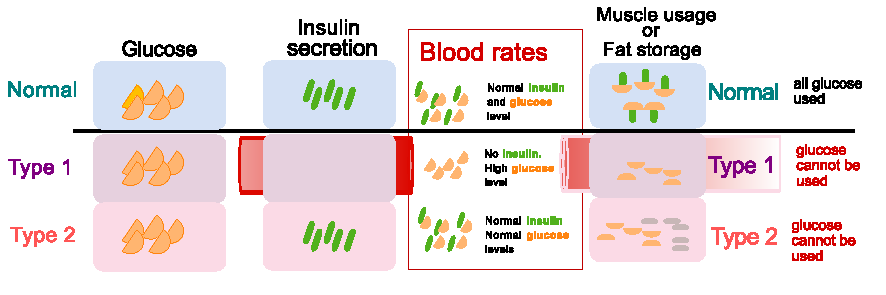
\includegraphics{diabetes_drawing}

\subsection{Objectives}
We want to address two issues: 
\begin{itemize}
\item Improve patient's education about his disease,
\item Raise the awareness of patient's entourage.
\end{itemize}
% IL MANQUE LA REF!!! ET IL FAUT INTRODUIRE LA CITATION: As XXX stated: blabla
\paragraph{} 
A lack of education about diabetes can have fatal consequences, leading in some cases to coma or death. In order to provide more effective for adolescent's education, we want to develop an interactive and adaptive software. Teaching experience can be improved by the use of 3 Dimensional interactive worlds, as they offer an Immersive experience to the user. Such as virtual reality, this kind of environments offers new possibilities for adaptive teaching methods, and their growing importance in motivational reinforcement have been recently studied by Ershow~\cite{virtual_reality}.

Our objective is to develop a tool where the user is an avatar that can be diabetic. In this 3D realistic world, it would be possible to see how diabetes affects the way patients live, work or do any other activity they usually do in real life. Patients can learn about their disease, and experiment several behaviours to get a better understanding. For this purpose, we want to add a diabetic avatar in an existing 3D world. 

\paragraph{}
% Normalement on met pas ca au debut, on commence par une lettre
3D worlds can also help to reach our second objective, linked with patient's entourage: even though family and friends have a huge impact in diabetes, there's an obvious need for education here because it's not possible that they all attend lectures in the hospital. Peers pressure is an especially relevant factor during adolescence, while patients can follow teens that aren't aware of the possible harmfulness of their activities~\cite{relatives}.
With this kind of universe, relatives, or anyone interested can use another avatar, and take part into the simulation. This might lead to a better understanding of their interactions with ill people, and the way diabetics live as well.

\section{Deliverable}
We want to produce a prototype that can be used at least by the hospital staff before the end of the project, e.g. in September. 
Then, we want to assess the ability of the tool to meet our expectations.


\subsection{Features}
The software will include features among these three categories, according to the time and planning changes:

\begin{itemize}
\item A teaching tool:
Images, videos or web pages can be displayed.
MCQ can also be used, and content can be added by the hospital staff.

\item Attractivity:
Users can communicate with other people at the simulation this day if it's done in the hospital, or with their friends by inviting them.
We can add adaptive content and can take into account the users' 'category' i.e. age, gender and other characteristics that might be relevant to determine which content to display.

\item Simulation:
An interface where main indicators are displayed, such as glucose, insulin level in the blood will be available. Then, we can run a simulation by "eating" something and looking at the indicators' evolution. 
A tour can be recorded, so a new user can follow a predefined route, where an overview of the main events a diabetic can go through is shown.

\end{itemize}

\subsection{Test}
After producing the prototype, we want to measure the impact of this tool in the education of teenagers. For this purpose, we will give multiple choice questions to the patients after they used the tool.
We will focus both on strict memorization performances, such as more concepts kept in mind by users, or a low forgetting rate, and on the attractiveness for the users. The tool must be able to adapt to the user, e.g. not delivering inappropriate content in the way it can be too complex to understand given the faculties of the user, or appear too childish for a teenager. Techniques from artificial intelligence are to be used, such as ontologies. However, building an accurate model of the student is not expected for this prototype. We need to reach a level of maturity that is acceptable according to the hospital staff expectations, and that matches our main modelling objectives.

% REFERENCE SUR LE SUJET E FRANCAIS : http://cat.inist.fr/?aModele=afficheN&cpsidt=14195630%


\subsection*{Achievability}
A comparison has already been done between several tools and technology that can be used, such as:
Unity3D,
Open Simulator,
Second Life,
Gaming libraries, such as pygame or the Lightweight Java Game Library,
or a mobile application. 
We chose Open Simulator for the development, as many features are already provided: communication with others, object modelling and creation, avatar and physical engine.
Technically, there is no excessively tricky technology or architecture to use.

\section{Planning}

There is a lot to learn about diabetes and patients daily life before being able to clarify my requirements. Therefore, the project depends a lot on the meetings with hospital staff. In addition, the large wide of techniques and subjects that could be covered in this project make it achievable only if I clearly restrict the scope.
However, we can state that the key features consists on these points :
\begin{itemize}
\item Creating a model for sugar and insulin evolution rates in the blood
\item Modelling a system of feeding with some food objects
\item Enabling the display of educational material in at least one teaching support
\item Building a few effects representing some diabetes symptoms
\end{itemize}

The planning is detailed in the Gantt chart in annex~\ref{chap:gantt}.
% dis lesquelles sont optionnelles

 \appendix
    \chapter{Gantt}
    \label{chap:gantt}
%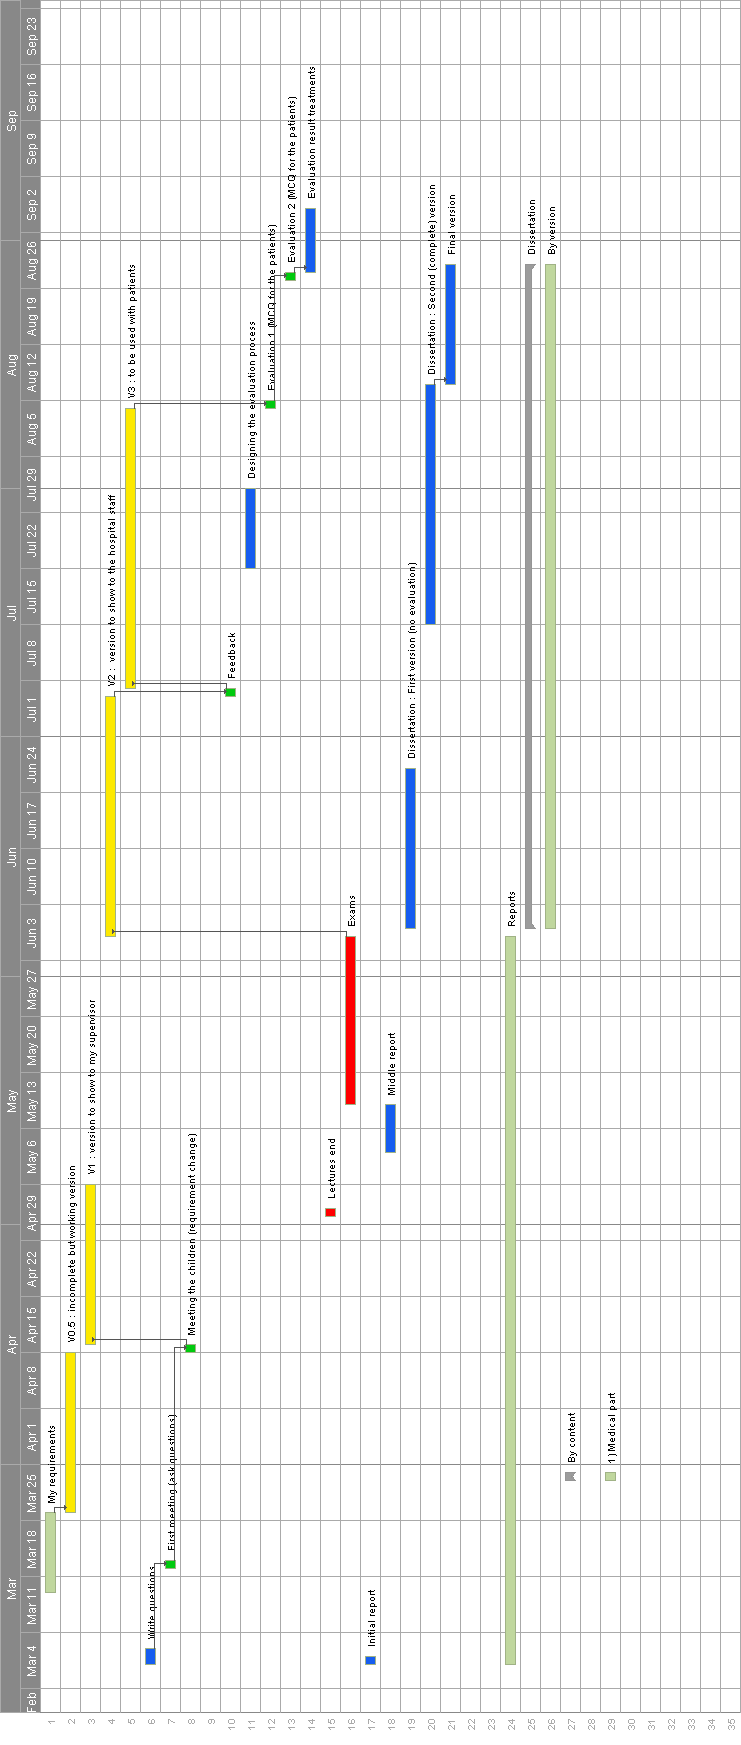
\includegraphics[scale=0.3]{GRANTT.png}
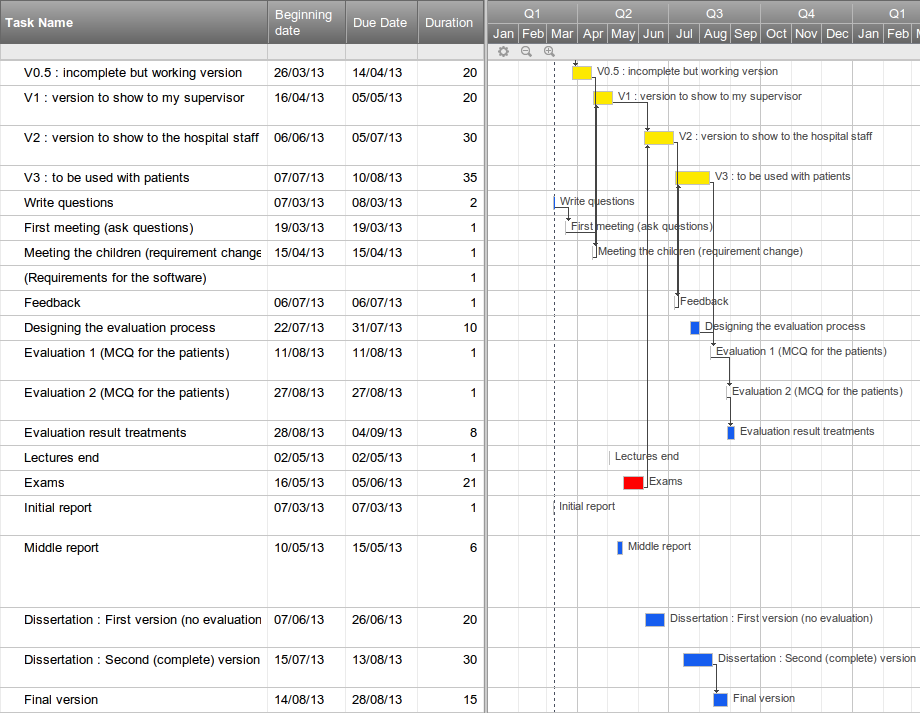
\includegraphics[scale=0.5]{HAN.png}
\fi


%%%%%%%%%%%%%%%%%%%%%%%%%%%%%%%%%%%%%%%%%%%%%%%%%%%%%%%%%%%%%%%%%%%%%%%%%%%%%%%%%%%%%%%%%%%%%%%%%%%%%%%%%%%%%%%%%%%%%%%%%%%%%%%%%%%%%%%%%%%%%%%%%%%%%%%%%%%%%%%%%%%%%%%%%%%%%%%%%%%%%%%%%%%%%%%%%%%%%%%%%%%%%%%%%%%%%%%%%%%%%%%%%%%%%%%%%%%%%%%%%%%%%%%%%%%%%%%%%%%%%%%%%%%%%%%%%%%%%%%%%%%%%%%%%%%%%%%%%%%%%%%%%%%%%%%%%%%%%%%%%%%%%%%%%%%%%%%%%%%%%%%%%%%%%%%%%%%%%%%%%%%%%%%%%%%%%%%%%%%%
    \bibliographystyle{alpha}
    \bibliography{mybib}
%eatwell plate picture: http://www.food.gov.uk/multimedia/pdfs/theeatwellplate.pdf

\end{document}
